\section{Espacio de trabajo y Paquetes}
\subsection{Estructura General}
Cuando utilizamos ROS 2, debemos organizar nuestras carpetas y archivos de una forma muy específica. De manera muy general, la organización va así: 

\textbf{espacio de trabajo}\textgreater\textbf{paquetes}\textgreater\textbf{nodos de ros}. 
\vspace{0.8em}

Un espacio de trabajo es una carpeta que contiene todas las carpetas y archivos de nuestro proyecto. Un paquete es una carpeta que contiene los nodos que programemos. Un nodo es un archivo de código fuente, usualmente un objeto.

Más detalladamente, la estructura de un espacio de trabajo de ros se ve así:

\vspace{1em}

\begin{center}
\begin{minipage}{1.1\textwidth}
\dirtree{%
.1 \textbf{ros2\_ws/} \dotfill Espacio de trabajo (\textit{Workspace}).
.2 \textbf{src/} \dotfill Directorio raíz del código fuente.
.3 \textbf{mi\_paquete\_cpp/} \dotfill Paquete de C++ (\textit{ament\_cmake}).
.4 CMakeLists.txt \dotfill Instrucciones de compilación de CMake.
.4 package.xml \dotfill Declaración de dependencias y metadatos.
.4 include/ \dotfill Archivos de cabecera (.hpp).
.4 src/ \dotfill Código fuente ejecutable.
.5 \textbf{nodo\_cpp.cpp} \dotfill Nodo escrito en C++.
.3 \textbf{mi\_paquete\_py/} \dotfill Paquete de Python (\textit{ament\_python}).
.4 package.xml \dotfill Declaración de dependencias y metadatos.
.4 setup.py \dotfill Configuración de instalación de Python.
.4 setup.cfg \dotfill Definición de ejecutables/puntos de entrada.
.4 mi\_paquete\_py/ \dotfill Módulo principal de Python.
.5 \textbf{nodo\_py.py} \dotfill Nodo escrito en Python.
.2 \textbf{build/} \dotfill Archivos intermedios (generado por \texttt{colcon}).
.2 \textbf{install/} \dotfill Puntos de entrada y binarios (generado por \texttt{colcon}).
.2 \textbf{log/} \dotfill Registros de depuración (generado por \texttt{colcon}).
}
\end{minipage}
\end{center}

\vspace{1.5em}

En el diagrama anterior, se muestra la estructura de un espacio de trabajo de ROS, con dos paquetes, uno de C++ y otro de Python.

\subsection{Creación de un Espacio de Trabajo}
Vamos a crear un espacio de trabajo en la terminal de Linux. Primero, creamos una carpeta que será el espacio de trabajo, a esta carpeta la nombraremos \texttt{taller\_ws} (nótese que \texttt{ws} viene de workspace o espacio de trabajo). Entonces creamos la carpeta con \texttt{mkdir taller\_ws}. 

\begin{verbatim}
usuario@equipo:~/ROS$ mkdir taller_ws
\end{verbatim}

Luego, dentro del espacio de trabajo crearemos una carpeta llamada \texttt{src} (esa carpeta por convensión se llama así).

\begin{verbatim}
usuario@equipo:~/ROS$ cd taller_ws
usuario@equipo:~/ROS/taller_ws$ mkdir src
\end{verbatim}

Dentro de \texttt{src}, vamos a hacer un paquete de C++ llamado \texttt{viz\_package\_cpp}. Queremos que este paquete contenga:

\begin{itemize}
    \item un archivo \texttt{CMakeLists.txt}
    \item una carpeta \texttt{include/}
    \item una licencia Apache 2.0
    \item un archivo \texttt{package.xml}
    \item una carpeta con un nodo \texttt{src/viz\_node.cpp} 
\end{itemize}

Lo anterior lo podemos hacer con el siguiente comando:

\begin{verbatim}
ros2 pkg create --build-type ament_cmake --node-name \
viz_node viz_package_cpp --license Apache-2.0
\end{verbatim}

\begin{center}
  \begin{Verbatim}[gobble=4]
    usuario@equipo:~/ROS/taller_ws$ cd src
    usuario@equipo:~/ROS/taller_ws/src$ ros2 pkg create --build-type ament_cmake \
    --node-name viz_node viz_package_cpp --license Apache-2.0
  \end{Verbatim}
\end{center}

\begin{figure}[H] 
  \centering    
  \makebox[\textwidth][c]{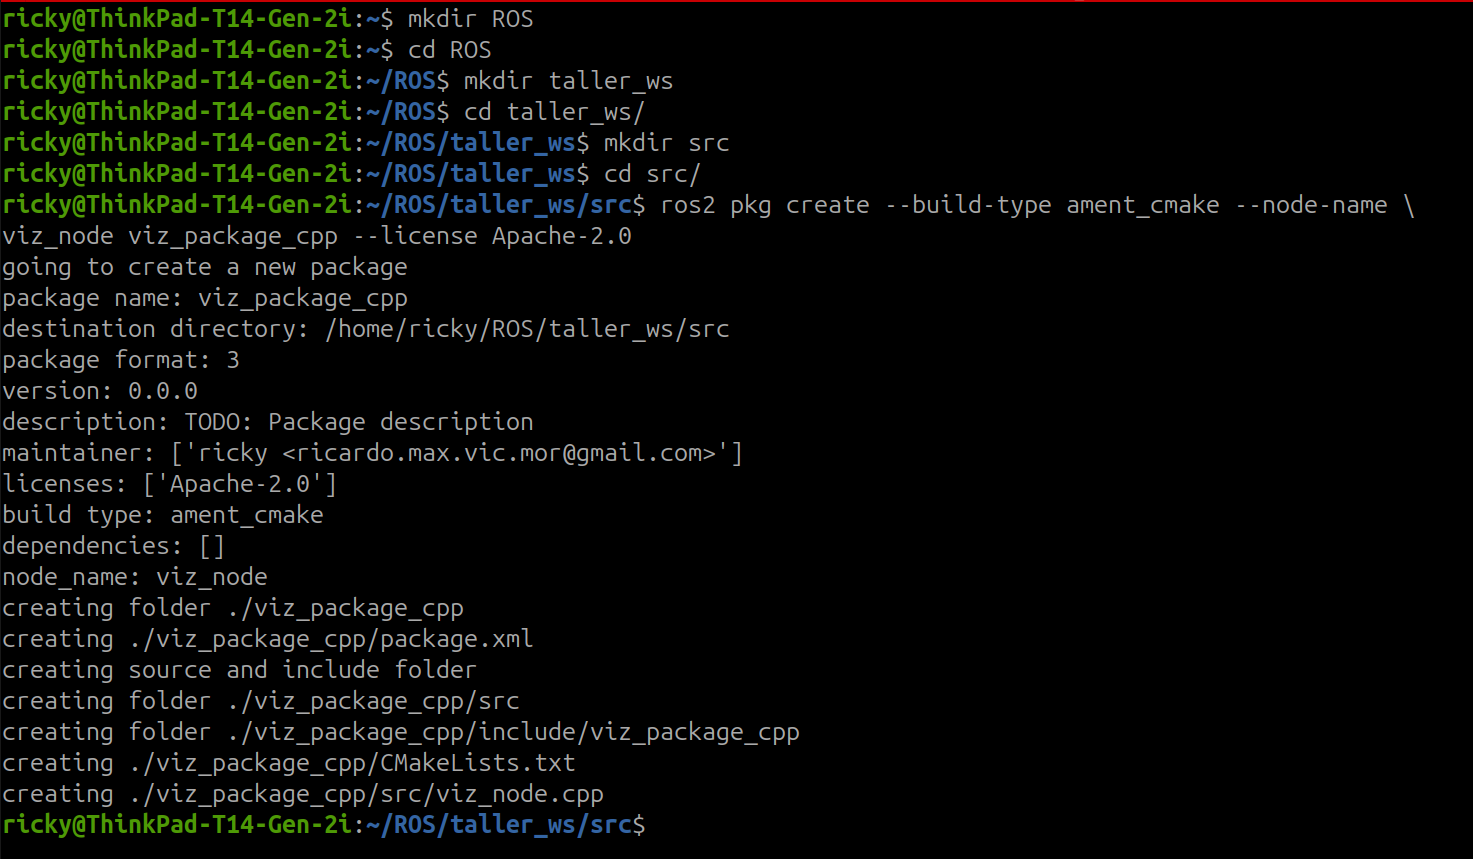
\includegraphics[width=1.4\textwidth]{imagenes/1.png}}
  \caption{Creación de Espacio de Trabajo, y Paquete con Nodo.}
  \label{fig:mi_imagen}
\end{figure}

A continuación se muestra cómo quedó la estructura del paquete.

\begin{center}
  \begin{Verbatim}[gobble=4]
    usuario@equipo:~/ROS/taller_ws/src$ tree
    .
    └── viz_package_cpp
        ├── CMakeLists.txt
        ├── include
        │   └── viz_package_cpp
        ├── LICENSE
        ├── package.xml
        └── src
            └── viz_node.cpp

    5 directories, 4 files
  \end{Verbatim}
\end{center}

\begin{figure}[H] 
  \centering    
  \makebox[\textwidth][c]{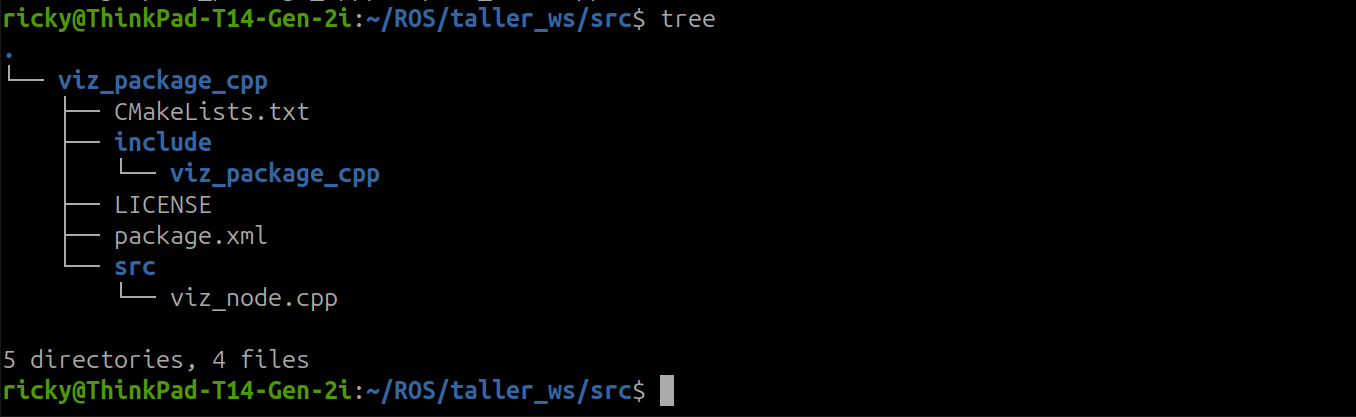
\includegraphics[width=1.4\textwidth]{imagenes/1-2.png}}
  \caption{Estructura del Paquete.}
  \label{fig:mi_imagen}
\end{figure}

[en otras iteraciones, explicaré el contenido de los archivos anteriores].

\subsection{Compilar y Ejecutar}
Una vez que tenemos la estructura que definimos anteriormente. Procedemos a compilar el espacio de trabajo, y ejecutar el nodo que creamos. El nodo que creamos anteriormente sólo devuelve un hola mundo. 

Para compilar, usamos \texttt{colcon}, la herramienta de compilación por línea de comandos oficial de ROS 2. Su función es orquestar la construcción de múltiples paquetes dentro de un espacio de trabajo.

Podemos compilar e instalar todo el espacio de trabajo con:

\begin{center}
  \begin{Verbatim}[gobble=4]
    colcon build
  \end{Verbatim}
\end{center}

o podemos compilar e instalar un paquete específico con:

\begin{center}
  \begin{Verbatim}[gobble=4]
    colcon build --packages-select <nombre del paquete>
  \end{Verbatim}
\end{center}

\begin{figure}[H] 
  \centering    
  \makebox[\textwidth][c]{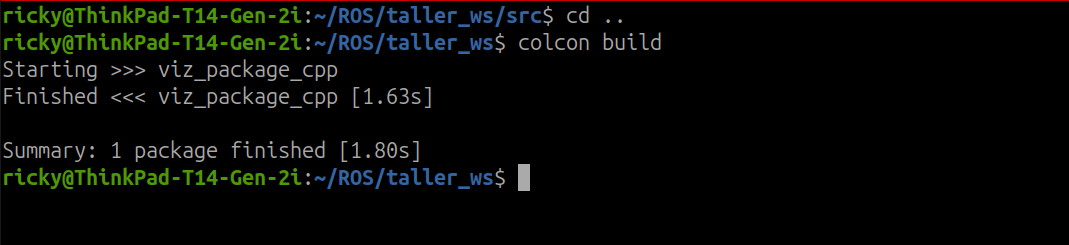
\includegraphics[width=1.4\textwidth]{imagenes/2.png}}
  \caption{Compilación.}
  \label{fig:mi_imagen}
\end{figure}

Luego, para ejecutar un nodo de un paquete, abrimos una nueva terminal (no se debe ejecutar en la misma terminal donde se compiló, porque puede fallar la ejecución), y en la nueva terminal activamos el overlay con:
\begin{center}
  \begin{Verbatim}[gobble=4]
    source install/local_setup.bash
  \end{Verbatim}
\end{center}
y ejecutamos el nodo con:
\begin{center}
  \begin{Verbatim}[gobble=4]
    ros2 run <nombre del paquete> <nombre del nodo>
  \end{Verbatim}
\end{center}

\begin{figure}[H] 
  \centering    
  \makebox[\textwidth][c]{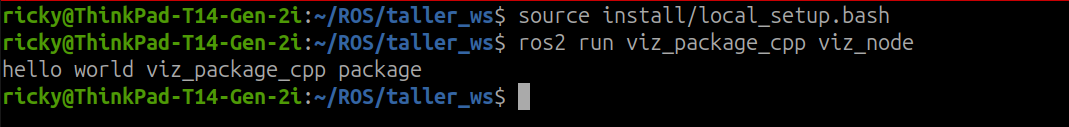
\includegraphics[width=1.4\textwidth]{imagenes/2-2.png}}
  \caption{Ejecución del Nodo.}
  \label{fig:mi_imagen}
\end{figure}